\documentclass[Softwaredesign/Softwaredesign_main.tex]{subfiles}
\begin{document}
\section{Design af RPiApp - USER SPACE}
\subsection{Indledning}
Beer Pong er et eventbaseret spil. Det omhandler masser af asynkrone handlinger; når der rammes ned i en kop, fjernelse af kop,  indsættelse af mønt mm. Det er således utrolig vigtig, at vores system kan opfange alle disse asynkrone events. Selvom alle handlingerne fra brugeren er asynkrone, ønsker vi stadigt at interagere med handlingerne sekventielt. Dette er en vigtig faktor, da hvis en bruger laver to eventhandlinger inden for en kort tidsramme, skal vi sikre at systemet når at reagere på begge handlinger. En af måderne for at opnå dette er reaktiv programmering: Vi ønsker at opdatere vores system med det samme brugeren interagere med det. 
\\Reaktiv programmering er dog blot en af de ting, som er nødvendigt for vores system. En anden er håndtering af de asynkrone events. Det skal sikres, at når en enhed er i en tilstand af foranding (fx en bruger har fjernet en kop), at dette håndteres korrekt. Der kan også opstå et tilfælde, hvor to enheder (fx Playerside 1 og 2) sender en asynkron besked til RPi samtidigt. Her skal det være muligt at afhandle begge beskeder. Dette problem kan løses ved 'event driven' arkitektur. \\\\
Softwareapplikationen RPiApp er udviklet objektorienteret i sprogen C++17.  Der vil være enkelte elementer fra C11, når enkelte klasser gør brug af i2c-kommunikation (Kræver kommunikation / operationer til Kernal Space, som kun findes i C). Hvis sproget afviger fra standard, vil det blive nævnt i afsnittet.
\subsection{Event driven arkitektur}
Et event drevet system reagerer ud fra signaler og tilstande fra aktører/delsystemerne\footnote{Delsystemer er repræsenteret i form af boundary klasserne i RPiApp} i systemet. 
Her bruges en bus til at håndtere events i en sekventiel orden, således intet går tabt eller bliver forstyrret af andre delsystemer. 
\\En måde at håndtere signalerne imellem delsystemerne er brugen af MsgQueue. MsgQueue er en klasse, som gør det muligt at sende og modtage brugerdefineret beskeder, uden de kan påvirkes, opfanges eller forstyrres af andre tråde eller lignende (Kun den tråd som behandler beskeden). De brugerdefinerede beskeder laves i form af nedarvninger af klassen Message. Beskederne kan designes, så de kan indeholde den information, vi ønsker, om det skal være en integer, objekt af klasse eller lignende.\footnote{MsgQueue og Message klasserne er udarbejdet i ISU-faget}. 
\\MsgQueue indeholder også et objekt af en STL Queue. Dette betyder at når en besked modtages er strukturen FIFO (First in, first out). Dette betyder, at selvom beskederne er asynkrone, så vil de behandles sekventielt i 'køen'. Hvert delsystem får et MsgQueue objekt, således de kan kommunikere med hinanden.

GameController er den klasse, som tager alle beslutninger for systemet. Alle boundary klasserne indsender deres data til GameControllers MsgQueue. Data behandles derefter i GameController. Klassen vil blive beskrevet længere ned i dokumentet. 
\\\\'Publisher og subscriber pattern' ville også have været en effektiv måde at behandle stadiehåndteringen. Her ville de forskellige boundary klasser 'abonnerer' på GameController klassen, som ville 'publicere' stadierne. Her ville den lokale MsgID håndtering være ideel, da hvert boundary klasse ville have deres egen måde at forstå stadiet på. GameController (publisher) ville udsende et globalt stadie. Hver boundary klasse ville udnytte/behandle denne information forskelligt. For eksempel Display og Playerside afspejler GameControllers stadier, men BallDispenser skal kun gøre noget i nogen af stadierne: den initierer spillet og angiver status af bolde (Empty / NotEmpty).
\\\\Dette kunne have været løst med et lokalt MsgId. Desværre blev termologien og teorien for dette mønster først lært sent i projektudviklingen, og bruges ikke i dette projekt. 

\begin{figure}[H]
    \centering
    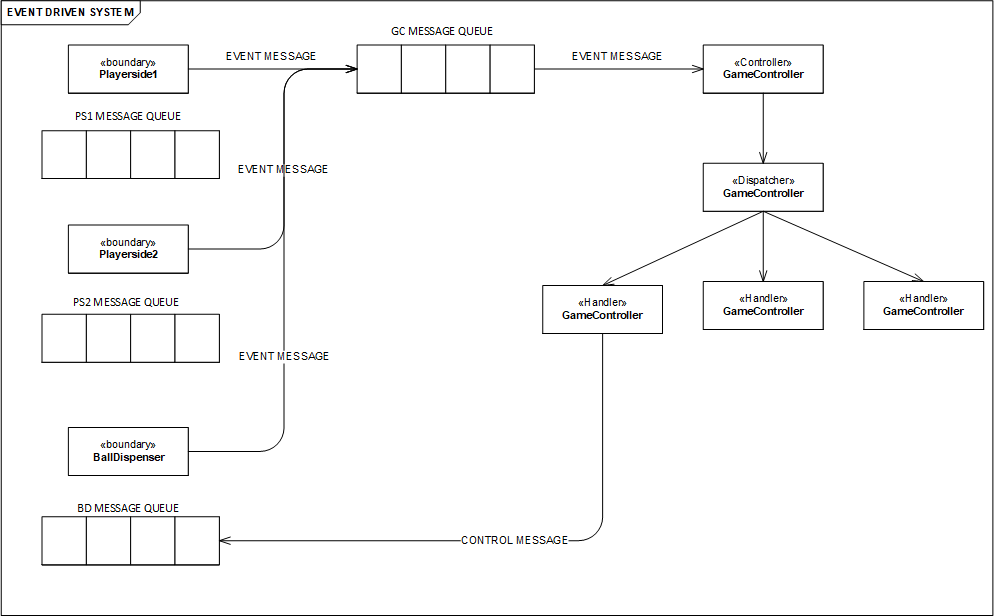
\includegraphics[width=0.8\textwidth]{Softwaredesign/RPiApp/graphic_RPi/EDS.png}
    \caption{Skitse af event drevet system - Producer / Consumer}
    \label{fig:EDS}
\end{figure}
\subsection{Resource Handling}
En af de vigtigste elementer ved brugen af MsgQueue-systemet er 'inter thread communictation', hvilke gør det muligt at behandle fælles data mellem tråde. Designet tager udgangspunkt i Producer / Consumer strukteren. Det kan ses på figur \ref{fig:EDS} at alle boundary klasser og controlleren har en tråd, som de bruger til at modtage data via deres MsgQueue objekt, deres buffer. Det essentielle i dette er, når en klasse vil sende en besked til en MsgQueue 'buffer, bliver det allokeret dynamisk, og når beskeden er afviklet af 'consumeren' bliver beskeden slettet. Dette betyder, at alle de dynamisk allokerede resourcer i beskeden bliver deallokeret - en ekstrem vigtig faktor, når flere hundrede beskder bliver behandlet mellem trådene. Alt sendt via MsgQueue er også trådsikret, da det er indkapslet i Mutex'er. 
\subsection{Delsystemer og tilhørende tråde}
For hver boundary klasse tildeles en tråd - for boundary klassen BallDispenser og Playerside tildeles en tråd til at læse og skrive. En bevirkning for funktionen readPlayerside() op readBallDispenser() er, at processen (og dermed tråden) sover, indtil et interrupt modtages.  
Vi ønsker stadig at kunne sende til Playerside og må derfor have en sideløbende tråd til at skrive til den. Alle tråde skal konstant checke deres MsgQueue objekt (Deres besked kø) for information. Når en besked modtages, afhandles den via en 'dispatcher'. Nedenfor ses et eksempel på en tråd.
\\Design example for thread function. \footnote{Idéen af dette design er taget fra ISU undervisning: Thread\_Communication}
\begin{lstlisting}[caption={Design af trådfunktion},label={lst:threadfuc}]
void * threadFunction(void *)
{
    while(systemisactive)
    {
        unsigned long id;
        Message * msg = MessageQueueObj_.recieve(id);
        Dispatcher(msg, id);
        delete msg; 
    }
}
\end{lstlisting}

\subsection{ThreadFunctor og Threads}
Alle boundary og controller klasser har en tilhørende tråd, som både er kommunikationen mellem klasserne, men også klassens egen måde til at håndtere beskeder og reagere på dem uafhængigt af andre tråde i systemet. Koden er designet ud fra et objekt orienteret princip. For at initialisere en tråd implementeres to klasser: ThreadFunctor og Thread. Begge klasser er inspireret fra ISU undervisningen \footnote{Lektion 6, indsæt link}. Den abstrakte klasse ThreadFunctor består af to funktioner: rent virtuel run() og threadMapper()
\\ThreadFunctor er base klassen til de funktioner, som ønsker at have have en tilknyttet tråd. Boundary klasserne skal derfor nedarve fra ThreadFunctor. 

Da funktionen run() er rent virtuel, skal den implementeres for de nedarvede klasser; den repræsenterer klassens trådfunktion. I form af ThreadFunctors pointer 'tf\_' tager den imod et nedarvet objekt af base klassen ThreadFunctor, som i dette tilfælde er den nedarvede klasse vi ønsker at bruge til tråde. 
\begin{lstlisting}[caption={threadMapper funktion},label={lst:threadmap}]
void * ThreadFunctor::threadMapper(void * thread)
{
	ThreadFunctor * tf = static_cast<ThreadFunctor*>(thread);
	tf->run();
	return nullptr;
}
\end{lstlisting}
Det skal dog nævnes at kreationen, 'joining' og nedlæggelse af tråden er ikke ThreadFunctors opgave men klassen Thread. Thread-klassen er en friendklasse i ThreadFunctor, således den har adgang til private og protected medlemmer af ThreadFunctor klassen. Dette betyder, at når vi skal bruger funktionen pthread\_create()\footnote{pthread.h biblioteket} så har vi adgang til 'trådfunktionen' for det nedarvede objekt via threadMapper. 
\begin{lstlisting}[caption={Udsnit af Thread-klasse},label={lst:thread}]
class Thread
{
...
private:
	ThreadFunctor * tf_;
	pthread_t threadId_;
	bool attached_;
	
//initialization 
pthread_create(&threadId_, nullptr, ThreadFunctor::threadMapper, tf_)
};
\end{lstlisting}
\subsection{Dispatchers og handlers}
En dispatcher er en 'overall' event handler. Den bruges til at håndtere den besked, som tråden modtager gennem dens besked kø. Der 'modtages' to parametre fra receive()-funktionen: et id som repræsenterer den service, handleren skal tilbyde, samt en besked som er en nedarvet brugerdefineret objekt af klassen Message (Den kan indeholde forskellige parametre i sig selv, hovedsageligt information som skal veksle mellem trådene). Ud fra parameteren 'id' vurderes hvilke service, som skal udføres. Dispatcheren 'aktiverer' derefter de korrekte event handlers og videregiver message, hvis dette er relevant. 

Event handlerne vil derefter kalde det specifikke funktioner for de enkelte boundary klasser til at opnå målet for den givne service. GameController klassen (og tråden) styrer logikken i systemet og vil sende beskeder ud til de andres beskedkøer - dette realiseres gennem eventhandlerne, som kalder de korrekte metoder. 
\begin{figure}[H]
    \centering
    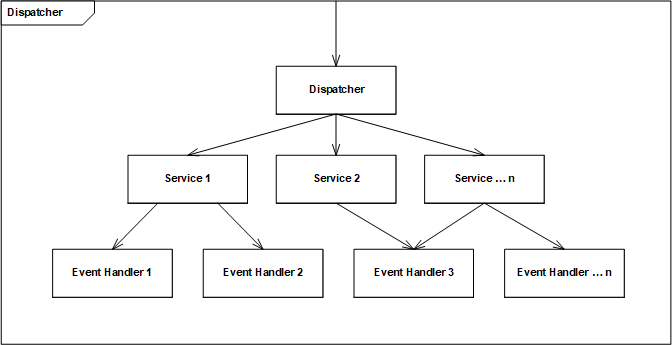
\includegraphics[width=0.8\textwidth]{Softwaredesign/RPiApp/graphic_RPi/dispatch.png}
    \caption{Skitse af dispatcher, services og eventhandlers (Version 1, ikke færdig, måske heller ikke så relevant)}
   \label{fig:dispatch}
\end{figure}
Nedenfor findes et kodeeksempel på en dispatcher og hvordan en id og beskeder afvikles: 
\begin{lstlisting}[caption={Dispatcher Design},label={lst:dispatch}]
void dispatcher(unsigned long MsgID, Message * msg)
{
    switch(MsgID) 
    {
        case SERVICE 1 :
        {
            EventHandler1(static_cast<InheritedMessageType *>(msg)); 
        }
        break;
        
        case SERVICE 2 : 
        {
            EventHandler2(); 
            EventHandler3(static_cast<InheritedMessageType *>(msg));
        }
        break;
        default : //Error handling
    }
}
\end{lstlisting}
\subsection{Oversigt}
Dette afsnit beskrev kort det overordnede design af kommunikationen mellem klasserne. Det vigtigste element for denne kommunikation er, at boundary klasserne ikke skal kunne få systemet til at afvige fra standarden (Use cases etc.). GameController klassen skal styre systemet og modtage beskeder gennem dets beskedkø. Alle beskeder afvikles sekventielt og er låst i form af mutexer. Dette er essentielt for systemet, da der ofte behandles delt data. 

\section{Opdateret klassediagram for RPi}
Da applikationen er designet ud fra event driven arkitektur, er der tilføjet flere klasser og metoder til systemet. I de følgende afsnit kan ses flere opdaterede klassediagrammer, hvor fundamentet er taget fra applikationsmodellen for RPiApp. Det er ikke noget overordnet klassediagram for systemet, da det ikke gav noget overskueligt billede af klassernes sammenhæng. \\\\
Systemet designes ud fra figur \ref{fig:dispatch}, og dette indebærer at de fleste funktionsnavne fra applikationsmodellen skifter navn til \textbf{handle[functionname]}. Dette er som sagt baseret på event driven arkitektur, og programmet skal 'handle' de forskellige beskeder modtaget fra boundary klasseren - fx "handleSystemIdle".  
\section{GameController - Controller}
\begin{figure}[H]
    \centering
    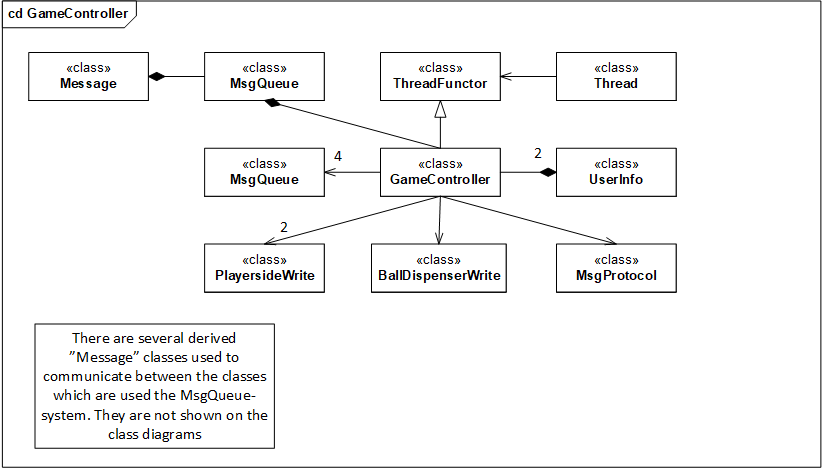
\includegraphics[width=1\textwidth]{Softwaredesign/RPiApp/graphic_RPi/GC.png}
    \caption{Klasse diagram for GameController}
   \label{fig:cd_GC}
\end{figure}
Controller-klassen er den som eksekverer use cases ved at interagere med boundary og domæne klasserne. Den indeholder alt logik og tager de fleste beslutninger. Til forskel fra den traditionelle stil, indeholder denne klasse en del stadier. Dette skyldes hovedsageligt kravspecifikation for systemet: Use case 1 til 3 er en forlængelse af hinanden, og derved samlet i en controller klasse 'GameController'. Dette betyder, at den skal initiere forskellige stadier i forhold til spillets gang og 'spilstadier'. Designet af dispatcheren for controlleren tager udgangspunkt i listing \ref{lst:dispatch}. Med det sagt, så var der flere valg i forhold til strukturen af dispatcheren. Hvis den kun tog udgangspunkt for MsgID til at vælge mellem hvilke 'service', som skal udføres, ville det give mulighed for at boundary klasserne kunne styre hvilke service, som skulle udføres, uafhængigt at den nuværende tilstand for spillet. For eksempel hvis beskeden "Coin Inserted" bliver sendt, imens spillet er i gang, vil klassen udføre en tilhørende service, som ikke burde kunne kaldes i det stadie. Vi valgte derfor at indsætte en ekstra switch-case, som er en funktion af stadiet for GameController. Herved kan man kontrollere, at kun 'godkendte' beskeder bliver afviklet i dispatcher/handler. 
\\\\En af ulemperne ved dette, er at de gør koden uoverskueligt og nested switches er generelt noget, man skal undgå. En anden ting man kunne have implementeret var dobbelt dispatching, hvor hver type besked har sin egen dispatcher og tilhørende handlers.
\\\\Hver MsgID-besked har sin egen handler. I enkelte tilfælde sender GameController beskeder til sig selv, for at initiere en ny tilstand og kalde tilhørende handler (Her modtager handleren ingen brugerdefineret 'Message' besked). Da beskederne afvikles sekventielt, vil tidligere beskeder eksekveres først. \\¨
Hvis en boundary klasse sender en MsgID og brugerdefineret besked til GameController afvikles begge argumenter i handleren (Typen af besked 'BallDispenserResponse' vil blive uddybet længere nede i afsnittet "Messages"): 
\begin{lstlisting}[caption={Design af handler},label={lst:bound_hand}]
handleBallDispenserResponse
(static_cast<BallDispenserResponse *>(msg)) 
\end{lstlisting}
%Nedenfor ses et udkast af designet af dispatcheren for GameController, listing \ref{lst:Game_Disp}. 
\begin{lstlisting}
void GameController::dispatcherGameMessage(unsigned long MsgID, 
Message * msg)
{
    switch(GameController state)
        case GAME_STATE_IDLE
            switch(MsgID)
                case COIN_INSERTED : 
                    handleBallDispenserResponse
                    (static_cast<BallDispenserResponse *>(msg)) 
                break;
        break; 
    ...
}
\end{lstlisting}
\\Til forskel for de andre klasser erklæres beskedkøen for GameController globalt. Dette gøres fordi alle boundary klasserne skal have adgang til den. \\\\
GameController modtager alt information fra de forskellige boundary klasse:
\begin{enumerate}
    \item \textbf{WebPage}: Holdnavn, Brugernavne og farvekoder
    \item \textbf{Playerside}: \textbf{Cups} status: hvilke kopper er blevet placeret og fjernet
    \item \textbf{BallDispenser}: Møntinsættelse og bolddispenser status (Tom eller ikke tom)
\end{enumerate}

\section{I2C}
I2C klassen er baseklassen for alt i2c-kommunikation. Ligeledes de andre klasser er den designet ud fra en objekt orienteret struktur, men den gør også brug af elementer fra C. I2C-klassen skal indeholder metoder, således det går det muligt at få tilgang til i2c-bussen og resourcer sendt vha. den - reelt set er det driveren, som håndtere alt information sendt og modtager via i2c-bussen, det er således i2c-klassens ansvar at kommunikere med driveren implementeret i kernal space. Her bruges filoperationer til at anvende kernal space interfacet. Til håndteringen af data og open/read/write-operationer bruges biblioteket "fcntl.h"\footnote{Open source library, gør det muligt at opererer på filer i Linux: http://pubs.opengroup.org/onlinepubs/000095399/basedefs/fcntl.h.html} \\\\
Klassen skal kun indeholde read og write operationenerne, det er den nedarvet klasses ansvar at få adgang til den specifikke fil (Alle filer er prædefineret). fx Playerside1 filen oprettes som "/dev/playerside1". Boundary klasserne "Playerside" og "BallDispenser"  gør brug af i2c kommunikationen og skal derfor nedarve fra denne klasse. Hvis flere metoder deles mellem klasserne, gøres de virtuelle og implementeres i de nedarvede klasser. 

\section{Playerside - Boundary}
\begin{figure}[H]
    \centering
    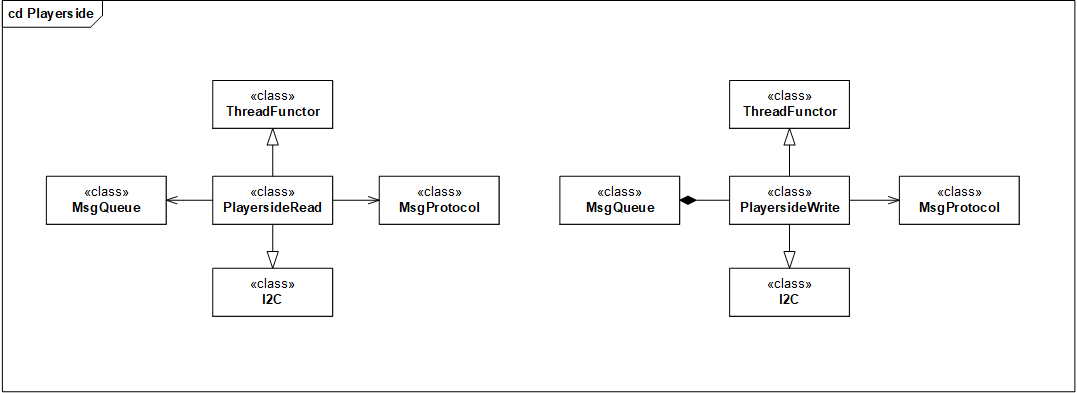
\includegraphics[width=1\textwidth]{Softwaredesign/RPiApp/graphic_RPi/PS.png}
    \caption{Klasse diagram for Playerside}
   \label{fig:cd_PS}
\end{figure}
Boundary klassen 'Playerside' er som nævnt i arkitekturen grænsefladen mellem PSoC'ene (For Pladerside 1 og 2) og RPi'en. I applikationsmodellen er Playersideklassen angivet som en klasse, som håndterer både 'read'- og 'write'-operationerne, men da begge operationer kræver en tråd, deles Playersideklassen op i to: "PlayersideRead" og "PlayersideWrite". 
\\\\Grunden til at hvert operationer kræver en tråd er, at 'read'-operationen får tråden til at 'sove' indtil et interrupt finder sted. Hvis tråden sover kan den ikke kalde 'write'-operationen, da den er 'låst'. Desuden når der nedarves fra klassen ThreadFunctor, skal den rent virtuelle metode run() implementeres, som implicit er tråden. Da kun en run()-metode kan implementeres 'per nedarvning', skal boundaryklassen deles i to. \\\\
Klassen nedarver også fra I2C klassen. Det er generelt dårlig praksis at nedarve fra flere klasser. Her kan opstå flere problemer, som kan skabe fatale konsekvenser for ens program - en fejl benævnes som "the deadly diamond of death", hvor en nedarvet klasse nedarver fra to klasser, som har den samme baseklassen. I det tilfælde, ved den ikke hvilke 'overridden' funktioner, som den skal vælge (Dette kan løses vha. af virtual arv). 

En anden design løsning var at opdele klassen til 3 klasser: PlayersideReadThread, PlayersideWriteThread, PlayersideI2C. Dette skaber også høj samhørighed, da hvert klasser har mindre funktionalitet.  
\\\\\textbf{PlayersideRead}
\\Klassen PlayersideRead bruger alle nødvendige operationer fra applikationsmodellen (Angiv ref), samt en pointer til GameControllers MsgQueue, så den kan sende beskeder til dens beskedkø. Ligeledes GameController-klassen nedarver den fra ThreadFunctor og bruger metoden run() til implementering af tråden.
\\Klassens hovedfunktioner er at modtage data fra I2C-driveren, behandle det og så sende det videre til GameController. Klassen kan siges at bestå af to dele: En del som skal håndtere den event driven arkitektur og en del som skal håndtere fillæsning (fra I2C-driver)
\\\\\textbf{Data modtaget fra RPi\_IF}
\\Data sendt fra RPi\_IF bliver sendt via I2C. Alt data via I2C bliver håndteret i I2C-driveren, som vækker den korrekte fil i forhold til hvilken PSoC, som har triggered interruptlinjen. Når et objekt af PlayersideRead initialiseres skal det associeres med den korrekt fil/node dannet af I2C-driveren (I2C-driveren coldplugges og alle noderne er angivet ved boot). Her bruges operationen \textbf{Open}('filename', O\_RDWR) til at modtage en filepointer til den specifikke fil. Denne filepointer bruges bl.a. til 'read'- og 'write'-operationer (Som kaldes fra I2C klassen). Alt data modtaget bliver gemt i en buffer og sendt videre til GameController via en pointer opbevaret i en brugerdefineret besked. 
\\\\\textbf{PlayersideWrite}
\\Klassen PlayersideWrite skal videresende stadierne givet fra GameController til RPi\_IF. Dette gøres ved brug af write-funktionen fra I2C base klassen. Til forskel for PlayersideRead har klassen ikke en pointer til GameControllers beskedkø. Der er ikke behov for at sende information til GameController, da dette ansvar er hos PlayersideRead.
\\Alle stadier, som sendes til RPi\_IF, er defineret i MsgProtocol (i form af unsigned char, se MsgProtocol afsnittet). Klassen modtager beskeder fra GameController gennem dens MsgQueue. Alle beskeder afvikles i dispatcheren, som kalder den korrekte handler - til forskel for applikationsmodellen, er der en handler til hvert stadie (fx "handleIdleRequest()"). Før var alt logikken og funktionalitet indkapslet i writePlayerside() og setState(). Ligeledes de andre klasser bruges handlers i stedet.
Alle 'handlers' afspejler et stadie, og sender dette stadie direkte til RPi\_IF: 
\begin{lstlisting}
 int PlayersideWrite::handIdleRequest()
{
    //'IDLE' er definret i MsgProtocol 
	char sendBuffer[8] = { IDLE };
	writePlayerside(sendBuffer, 1);
	return 0;
}
\end{lstlisting}
Hver Playerside skal have en read og en write tråd, dvs der skal oprettes et PlayersideRead og PlayersideWrite objekt til hver Playerside enhed. Når et objekt oprettes, skal det associeres med den korrekte fil oprettet af driveren, og da driveren er coldplugget kender vi allerede filernes navne ("/dev/playerside1" og "/dev/playerside2"): 
\begin{lstlisting}
    PlayersideWrite ps1_w("/dev/playerside1");
\end{lstlisting}
\section{Messages (Brugerdefineret beskeder)}
Da de forskellige klasser bruger MsgQueue-systemet til at kommunikere med hinanden, kræver det, at man har mulighed for at definere, hvad beskeden skal indeholde af data. Dette gøres ved at lave en nedarvet klasse af 'Message', som indeholder den data, som skal sendes til en beskedkø. Alle beskeder som sendes bliver dynamisk allokeret og modtager sletter beskeden, efter den er afviklet (Lidt a la 'shoot and forget'). Når beskeden skal afvikles i handleren bruges static\_cast til at konvertere til den korrekte typebesked (som set i listing \ref{lst:Game_Disp}). Da static\_cast bruger er det ekstremt vigtigt, at ikke at allokere en forkert beskedtype af Message. Hvis denne besked behandles forkert vil det med garanti resulterer i segmentation fault. Her bruges det medsendte 'MsgID' til at tilkendegive beskedens type. \\\\
Eksempel på Dynamisk allokeret brugerdefineret besked
\begin{lstlisting}
MsgQueue_.send(MsgID, new UserDefinedMsg(inputarg1, inputargt2));
class UserDefinedMsg : public Message
{
public:
    UserDefinedMsg(inputarg1, inputarg2)
    ...
}
\end{lstlisting}
\section{MsgProtocol.h}
Domæneklassen MsgProtocol indeholder alle MsgID'er, som de forskellige klasser gør brug af (Her bruges 'enumeration' til at lave beskedid'erne). Alle boundary klasserne kender til denne klasse. Det ville være et bedre design valg at lave en domæne klasse for hvert klasse, som gør brug af MsgQueue systemet, da klasserne ikke behøver at kende til hinandens MsgId'er. Men da systemet allerede er ved at blive stort og abstrakt, samles alle 'enum' MsgId'erne og 'unsigned char' protokolbeskedere. \\\\
Det skal defineres tydeligt, hvilke klasses MsgId eller protokolbesked som behandles.

\section{BallDispenser - Boundary}
\begin{figure}[H]
    \centering
    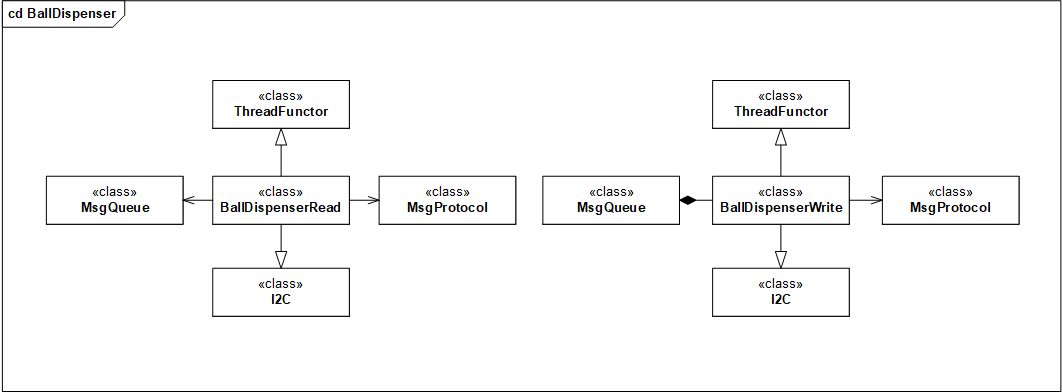
\includegraphics[width=1\textwidth]{Softwaredesign/RPiApp/graphic_RPi/BD.png}
    \caption{Klasse diagram for BallDispenser}
   \label{fig:cd_BD}
\end{figure}
Boundary klassen BallDispenser er grænsefladen mellem BallDispenser-enheden og RPi. Ligeledes for Playerside klassen, skal klassen opdeles til to klasser, da write og read operationerne kræver to tråd: BallDispenserRead og BallDispenserWrite. Som det kan ses på figur \ref{cd_BD}, har klassen samme struktur som PlayersideWrite og PlayersideRead. BallDispenserRead og -Write henter informationer omkring MsgId'er og protokolbeskder for MsgProtocol domænet. 

\section{UserInfo - Domæne}
UserInfo er systemets database for brugeren; Holdnavn, spillernavne, antal kopper tilbage, holdfarve og modtstanderfarve. Der oprettes to instanser i GameController, som bruges til de logiske operationer i systemet - når det registeres at en kop er blevet fjernet for hold 1 (Playerside1), gemmes denne information i den instans svarene til hold 1. GameController bruger her instanserne til fx at checke om alle kopper er blevet placeret. \\
Instanserne initialiseres med default argumenter for brugeroplysningerne, da de først gives ved interaktion med WebPage klassen. Instanserne passeres dynamisk mellem klasserne GameController og WebPage. For at sikre at resourcerne bliver allokeret og frigivet korrekt, så anvendes 'rule of three' (destructor, copy constructor, copy assignment operator). 

\section{WebPage - Boundary}
\subsection{Indledning}
Dette afsnit omhandler boundary-klassen WebPage. I Beer Pong bordets RPi er der installeret en Apache web server. Det er en populær web server applikation, som gør det muligt at hoste hjemmesider. Serveren kan hoste HTML filer med det formål at vise informationer, men forskellige script-sprog kan også tages i brug. Det giver mulighed for at lave en dynamisk hjemmeside, som tilbyder mere interaktion og kommunikation mellem bruger og klientsiden. I vores projekt designes en hjemmeside, som skal modtage nogle brugerinputs og videreformidle dem til resten af systemet. Mere specifikt får brugerne mulighed for at tilgå hjemmesiden via PC eller smartphone, hvor der kan indtastes holdnavne, brugernavne og holdfarver. Under spillet vil de fremgå af et display. Det giver en ekstra dimension til spillet, at brugeren selv kan angive sine oplysninger, og denne form for interaktion bør resultere i en forbedret brugeroplevelse. WebPage anvendes i denne forbindelse som en samlet betegnelse for alt, hvad der har med hjemmesiden at gøre. I virkeligheden består klassen af en klientside og en serverside, som kommunikerer internt gennem et WebSocket API. Formålet med dette afsnit er at forklare de overvejelser og valg, der ligger bag designet og at beskrive, hvordan kommunikationen forløber mellem de forskellige undersystemer.
\subsection{Websocket}
Normalt taler man om et request-response forhold mellem client og server. F.eks. kan en web browser være client og en applikation, som hoster en hjemmeside kan være server. Kommunikationen mellem dem anvender da HTTP, der fungerer som en request-response protokol. Web kommunikationen forløber typisk ved, at client sender en HTTP request eller anmodning til serveren. Denne svarer igen med et response eller svar besked, som både kan indeholde status information og andet indhold, der er anmodet om.\footnote{https://en.wikipedia.org/wiki/Hypertext\_Transfer\_Protocol} Typisk vil det foregå synkront, men request-response forholdet kan også implementeres asynkront, så svaret returneres på et ukendt senere tidspunkt. Det fremgår, at det er client, som sender en besked, og at serveren responderer herpå. Det er således altid client, der initierer kommunikationen, og kommunikationsformen kan betegnes som pulled.\footnote{Slides - Getting started with WebSockets}
\\Ved at opdatere HTTP forbindelsen til en WebSocket kan vi etablere en vedvarende forbindelse mellem client og server. WebSocket protokollen giver mulighed for at sende indhold til client uden at denne først har sendt en forespørgsel. Beskeder kan altså sendes frem og tilbage mellem client og server over en enkelt TCP port, mens forbindelsen holdes åben. Vi opnår dermed et push/pull forhold mellem client og server, hvor kommunikationen er full-duplex, og graden af overhead er sænket. \footnote{https://en.wikipedia.org/wiki/WebSocket} For at starte WebSocket forbindelsen foretages først et HTTP handshake bestående af en request og response, hvorefter forbindelsen opdateres fra HTTP til WebSocket.
\\ WebSocket API er beskrevet ved et JavaScript interface.\footnote{https://www.tutorialspoint.com/html5/html5\_websocket.htm} Der erklæres først et egentligt WebSocket objekt på følgende vis:
\begin{lstlisting}
    var Socket = new WebSocket(url, [protocal] );
\end{lstlisting}
Første argument er den URL, der skal forbindes til, og andet argument er en valgfri sub-protokol, der ikke anvendes i vores tilfælde. De fire events som er associeret med WebSocket objektet er beskrevet i tabellen nedenfor.
\begin{table}[H]
\centering
\begin{tabular}{|L{0.15\textwidth}|L{0.25\textwidth}|L{0.3\textwidth}|}
\hline
\textbf{Event} & \textbf{Event handler} & \textbf{Beskrivelse} \\ \hline
open & Socket.onopen & Eventet sker, når forbindelsen oprettes \\ \hline
message & Socket.onmessage & Eventet sker, når client modtager data fra server \\ \hline
error & Socket.onerror & Eventet sker, når der er en fejl i kommunikationen \\ \hline
close & Socket.onclose & Eventet sker, når forbindelsen lukkes \\ \hline
\end{tabular}
\caption{WebSocket events}
\label{tab:websocket_events}
\end{table}
Desuden er der to metoder, som kaldes på objektet. Send(data) transmitterer data over forbindelsen, mens Close() lukker forbindelsen.
\\I designet af WebPage er der særligt taget udgangspunkt i biblioteket uWebsockets\footnote{https://redmine.ase.au.dk:443/devs/development-kits/raspberry-zero/uwebsockets.git} og slides fra Websocket workshop\footnote{https://blackboard.au.dk/bbcswebdav/pid-1980963-dt-content-rid-5612561_1/courses/BB-Cou-UUVA-78527/WebSocketsGettingStarted.pdf}. Sidstnævnte beskriver fremgangsmåden for, hvordan biblioteket libuv gøres tilgængeligt både i kompileren og på RPi.
\subsection{Client}
Client definerer hjemmesidens interface, og den er implementeret som et HTML dokument. Der anvendes HTML og lidt CSS til at beskrive, hvordan hjemmesiden skal præsentere sig i browseren. Derudover er der anvendt JavaScript til at implementere WebSockets API beskrevet i forrige afsnit. Under initieringen oprettes Websocket objektet:
\begin{lstlisting}
    websocket = new WebSocket(ws://10.9.8.2:3000/);
\end{lstlisting}
Det fremgår, at der forbindes til URL 10.9.8.2, og at portnummeret er 3000. Når data skal sendes mellem client og server skal det være i tekstformat, eventuelt ved hjælp af JSON. JSON formatet anvendes til at konvertere JavaScript objekter til tekst, så data let kan sendes uden, at der skal foretages komplicerede operationer for at splitte og oversætte det. I vores tilfælde er det tekststrenge, som skal sendes fra client til server, nemlig brugernavne, holdnavne og holdfarver for team1 og team2. Derfor vurderes det, at den enkleste løsning er at konkatenere denne info og sende det som en samlet tekststreng. Dette varetages af funktionen acquireInfo(), hvoraf et udsnit er vist nedenfor. Der er implementeret en 'Start'-knap på hjemmesiden, som kalder funktionen, når der klikkes.\\
\begin{lstlisting}
<button type="button" onclick="acquireInfo()">Start</button>
\end{lstlisting}
\begin{lstlisting}
 function acquireInfo()
 {
    username1 = document.getElementById("username1").value;
    ...
    color1 = document.getElementById("color1").value;
    ...
    teamname2 = document.getElementById("teamname2").value;
    gameInformation = username1+'-'+color1+'-'+...+
    '-'+teamname2+'#';
    websocket.send(gameInformation);
  }
\end{lstlisting}
Det fremgår at inputs konkateneres til én tekststreng gameInformation. De adskilles med bindestreger, mens symbolet '\#' terminerer den. Herefter sendes det til serveren, ved at send() funktionen kaldes på websocket objektet med gameInformation som parameter.
\\Derudover er handlers beskrevet i tabel \ref{tab:websocket_events} implementeret. Onopen, onclose og onerror udskriver blot ''CONNECTED'', ''DISCONNECTED'' og ''ERROR'' i browseren. Onmessage informerer om at info er ''RECEIVED'' og kalder eventuelt close() på websocket.
\subsection{Server}
Serversiden er implementeret som en c++ klasse kaldet WebPage. Den har til opgave at lytte på port 3000, og når der er genereret et event, dvs. der modtages data fra client, kaldes event handleren onMessage. Funktionaliteten af onMessage defineres i funktionen WSInit(), og det er den, som er mest interessant i denne sammenhæng. Når tekststrengen modtages, skal denne indlæses i en buffer og separeres på passende vis. Hertil udnyttes biblioteket <sstream> og det faktum, at vi har angivet '-' som delimiters og '\#' som terminering.\footnote{https://stackoverflow.com/questions/5757721/use-getline-and-while-loop-to-split-a-string} \\Brugerinputs opbevares i første omgang i en STL container, og disse skal videresendes til GameController klassen. Der anvendes en separat klasse UserInfo, som indeholder alle relevante holdinformationer. Det indbefatter et holdnavn, to brugernavne, en holdfarve og antallet af kopper placeret i Playerside. Derudover er der implementeret passende set- og get-metoder for disse. WebPage har to UserInfo objekter team1\_ og team2\_ som members og disse kan nu initaliseres til passende værdier. \\\\For at sende disse til GameController klassen, anvendes systemet med Messages og MsgQueues, som er beskrevet tidligere. Det kræver imidlertid at WebPage har kendskab til GameControllers MsgQueue, så den har foruden de to UserInfo objekter også en pointer til denne som private member. GameController har ikke kendskab til WebPage's MsgQueue, da kommunikationen bevidst er gjort envejs. Hvis for eksempel GameController først sendte en request, for så at modtage objekterne i en response besked, kunne der hurtigt opstå komplikationer, hvis brugeren sendte oplysninger flere gange, dvs. der blev genereret gentagne events. Eksempelvis kunne der blive sendt en request, eller GameController kunne være ved at kopiere objekterne samtidig med, at WebPage modtog nye informationer. Der blev forudset problemer med race conditions og problematisk adfærd. Ved at gøre kommunikationen envejs og så simpel som mulig ('shoot-and-forget'), undgås dette, og det sikres, at gameController altid arbejder på de nyeste brugerinputs.
\\\\Der sendes nu en Message til GameControllers MsgQueue kaldet WebPageResponse. Den sendes med MsgID ID\_INFO\_READY og indeholder team1\_ og team2\_. Endelig sendes der en respons til client ved at kalde WebSocket metoden send() på ws objektet. For at opsummere er WSInit() funktionen beskrevet med pseudokode nedenfor. OnMessage funktionen kaldes for et Hub objekt h, som er en del af uWS biblioteket. Det fremgår desuden, at onMessage er implementeret som et lambda udtryk. Det betyder, at den skrives som en inline-funktion, som kan udføres umiddelbart efter, at den er defineret. Capture listen [\&] tillader, at den kan tilgå alle variabler i det scope, den er omgivet af.\footnote{https://www.geeksforgeeks.org/lambda-expression-in-c/}
\newpage
\begin{lstlisting}
void WebPage::WSInit() {
h.onMessage([&](char *message, size_t length, ..) {
    read message into buffer
    split string into substrings (tokenize)
    store substrings in STL container
    set team1_ and team2_
    create WebPageResponse
    send WebPageResponse to GameController MsgQueue
    send response to client
    }
 }
\end{lstlisting}
Det er forsøgt at give et overblik over modulet WebPage med et sekvensdiagram i figur \ref{fig:WebPage_sd}. Det viser, at brugeren interagerer med client, når der skal indtastes holdoplysninger, mens client og server kommunikerer gennem et WebSocket API, som tidligere beskrevet. Serveren benytter sig af klassen UserInfo og sender to objekter af denne til GameController klassen.  
\begin{figure}[H]
    \centering
    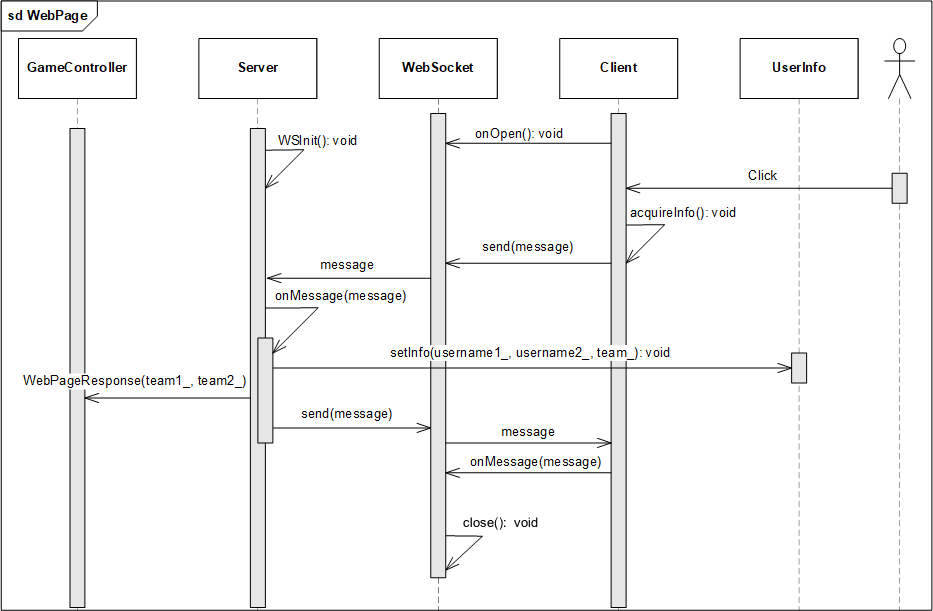
\includegraphics[width=1\textwidth]{Softwaredesign/RPiApp/graphic_RPi/WebPage_sd_2.png}
    \caption{Sekvensdiagram for WebPage}
    \label{fig:WebPage_sd}
\end{figure}

%%Skal måske med i design 
%Intro

%Arkitektur

%Klassebeskrivelser for GameController, Playerside, BallDispenser, WebPage? 

%Enumerationsbeskrivelser for MsgProtocol

\end{document}